\pdfminorversion=4
\documentclass[presentation, aspectratio=54]{beamer}

\usepackage[utf8]{inputenc}
\usepackage[T1]{fontenc}
\usepackage{fixltx2e}
\usepackage{graphicx}
\usepackage{float}
\usepackage{wrapfig}
\usepackage[normalem]{ulem}
\usepackage{amsmath}
\usepackage{textcomp}
\usepackage{amssymb}
\usepackage{hyperref}
\usepackage{tikz}

\tolerance=1000
% Include this file for dark background SUTD style
% Nils Ole Tippenhauer, SUTD, 2014
% This is somewhat hackish right now. Should be transformed into proper beamer theme
\mode<presentation>

\usecolortheme{rose}
\useinnertheme{rounded}
\usecolortheme{dolphin}
\useoutertheme{infolines}

% more stuff from Boadilla sty
\setbeamersize{text margin left=1em,text margin right=1em}
\setbeamertemplate{headline}[default] % disables headline
%\mode
%<all>

% disable tool bar
\beamertemplatenavigationsymbolsempty

% Logo
%\usepackage{pgf}  
%\logo{\pgfputat{\pgfxy(-1,8.32)}{\pgfbox[center,base]{\includegraphics[height=0.6cm]{./SUTD_logo_eng_hor_rev}}}}

% Fonts
\usepackage{helvet}
\usepackage{times} % for the serif stuff

% Title page, simple version
\setbeamertemplate{title page}{
%{\usebeamerfont{subtitle}\insertsubtitle\\}
 \usebeamerfont{title}\LARGE\bf\inserttitle\hrule
 \vspace{0.1cm}
 \usebeamerfont{author}\hfill\insertauthor
}
% for later: 
% \usebeamerfont{subtitle}, \insertsubtitle
% \usebeamerfont{institute}, \insertinstitute
% \usebeamercolor[fg]{titlegraphic}, \inserttitlegraphic
% \usebeamerfont{author}, \insertaddress

% hline for the titles
\setbeamertemplate{frametitle}{\usebeamerfont{title}\bf\insertframetitle\par\vskip-6pt\line(1,0){290}}

% now the colors
\definecolor{SUTDred}{RGB}{153,0,51}
\definecolor{lgrey}{RGB}{204,204,204}
\definecolor{mgrey}{RGB}{102,102,102}
\definecolor{dgrey}{RGB}{51,51,51}
\definecolor{Dgrey}{RGB}{37,37,37}%from the SUTD PowerPoint Template
\definecolor{white}{RGB}{255,255,255}

\setbeamercolor{normal text}{fg=white,bg=Dgrey}

\setbeamercolor{section number projected}{fg=white}
\setbeamercolor{section in toc}{fg=white}

\setbeamercolor{alerted text}{fg=SUTDred}

\setbeamertemplate{footline}{
   \begin{beamercolorbox}[ht=4ex,leftskip=0.2cm,rightskip=.2cm]{footer line}
    \hrule
    \vspace{0.1cm}
    \insertauthor \hspace{0.2cm} \inserttitle /\insertsection \hfill \insertdate\hspace{0.2cm}\insertframenumber\,/\,\inserttotalframenumber
    \vspace{0.1cm}
 \end{beamercolorbox}
}

\setbeamercolor*{item}{fg=white}
\useitemizeitemtemplate{\Large\raise-1.0pt\hbox{\textbullet}}
\usesubitemizeitemtemplate{%
    \tiny\raise1.5pt\hbox{$\blacktriangleright$}%
}
\usesubsubitemizeitemtemplate{\large\raise-1.0pt\hbox{\textbullet}}

\setbeamercolor*{palette primary}{fg=black,bg=white}
\setbeamercolor*{palette secondary}{fg=black,bg=mgrey}
\setbeamercolor*{palette tertiary}{fg=white,bg=black}
\setbeamercolor*{palette quaternary}{fg=white,bg=black}

\setbeamercolor{title}{fg=white}
\setbeamercolor{frametitle}{fg=white}
\setbeamercolor{framesubtitle}{fg=white}
\setbeamercolor{caption}{fg=white}

%\setbeamercolor{block title}{fg=white,bg=dgrey}
%\setbeamercolor{block body}{fg=black,bg=lgrey}
% test invisible blocks
\setbeamercolor{block title}{fg=white,bg=Dgrey}
\setbeamercolor{block body}{fg=white,bg=Dgrey}

% \setbeamercolor{block title alerted}{parent=alerted text,bg=black!15}
\setbeamercolor{block title alerted}{fg=white,bg=dgrey}
\setbeamercolor{block body alerted}{fg=black,bg=lgrey}
\setbeamercolor{block title example}{fg=white,bg=dgrey}
\setbeamercolor{block body example}{fg=black,bg=lgrey}

% enumerate
%\setbeamertemplate{enumerate items}[circle]
\setbeamercolor{enumerate items}{fg=black}
\setbeamertemplate{enumerate items}[square]
\setbeamercolor{item projected}{fg=black, bg=white}

\usepackage{textgreek}
\usetheme{default}

\definecolor{orchid}{RGB}{153, 102, 255}
\newcommand{\cyan}[1]{\textcolor{cyan}{#1}}
\newcommand{\magenta}[1]{\textcolor{magenta}{#1}}
\newcommand{\purple}[1]{\textcolor{orchid}{#1}}

\newcommand{\dhe}{\texttt{DHE}}
\newcommand{\dheexport}{\texttt{DHE\_EXPORT}\,}
\newcommand{\clienthello}{\texttt{ClientHello}\,}
\newcommand{\serverhello}{\texttt{ServerHello}\,}
\newcommand{\clientkex}{\texttt{ClientKeyExchange}\,}
\newcommand{\serverkex}{\texttt{ServerKeyExchange}\,}
\newcommand{\finished}{\texttt{Finished}\,}

\author{Asher Toback and Ben Hamlin}
\date{May 31, 2018}
\title{Imperfect Forward Secrecy \\ by David Adrian et al.}
\begin{document}

\maketitle

\section{Introduction}

%%%%%%%%%%%%%%%%%%%%%%%%%%%%%%%%%%%%%%%%%%%%%%%%%%%%%%%%%%%%%%%%%%%%%%%%%%%%%%%

\begin{frame}{Motivation}

Diffie-Hellman (DH): used for key exchange in
\begin{itemize}
\item TLS
\item SSH
\item SMTP
\item IKE (IPSec)
\item ...
\end{itemize}
\pause
\vspace{20pt}
Is it secure in practice?

\end{frame}

%%%%%%%%%%%%%%%%%%%%%%%%%%%%%%%%%%%%%%%%%%%%%%%%%%%%%%%%%%%%%%%%%%%%%%%%%%%%%%%

\begin{frame}{Contributions}

The authors...
\begin{itemize}
\item use zmap to explore the DH ecosystem
\item present a novel DH downgrade attack on TLS (logjam)
\item implement an attack on integer DH that's well-known in the literature, but
      unevaluated in practice (index calculus)
\item evaluate their attack on DH with small moduli and extrapolate its
      performance on bigger moduli
\end{itemize}

\end{frame}

%%%%%%%%%%%%%%%%%%%%%%%%%%%%%%%%%%%%%%%%%%%%%%%%%%%%%%%%%%%%%%%%%%%%%%%%%%%%%%%

\begin{frame}{Conclusions}

They conclude that...
\begin{itemize}
\item index calculus can break DH for a particular 512-bit modulus in time
      that's well within the reach of modern attackers
\item attackers with more resources may be able to break (may have broken) 768-
      and 1024-bit DH
\item moduli are often used on many hosts: an attacker could break DH for many
      hosts at once
\item many hosts/applications still allow 512-bit Diffie-Hellman, and downgrade
      attacks are possible
\item some hosts use unsafe misconfigured DH (e.g., $\frac{p-1}{2}$ is composite)
\end{itemize}

\end{frame}

%%%%%%%%%%%%%%%%%%%%%%%%%%%%%%%%%%%%%%%%%%%%%%%%%%%%%%%%%%%%%%%%%%%%%%%%%%%%%%%

\begin{frame}{Takeaways}

\begin{itemize}
\item Broken crypto is bad, mkay?
\item Use at least 1024-bit DH. (Use EC-based DH, if possible.)
\item Don't reuse moduli.
\item Beware of misconfiguration. (Don't roll your own crypto.)
\end{itemize}

\end{frame}

%%%%%%%%%%%%%%%%%%%%%%%%%%%%%%%%%%%%%%%%%%%%%%%%%%%%%%%%%%%%%%%%%%%%%%%%%%%%%%%

\section{Background}

%%%%%%%%%%%%%%%%%%%%%%%%%%%%%%%%%%%%%%%%%%%%%%%%%%%%%%%%%%%%%%%%%%%%%%%%%%%%%%%

\begin{frame}{Diffie-Hellman}

\cyan{Alice} and \magenta{Bob} want to do some symmetric crypto. They need a
shared \purple{key}. But their communication channel is public...

\end{frame}

%%%%%%%%%%%%%%%%%%%%%%%%%%%%%%%%%%%%%%%%%%%%%%%%%%%%%%%%%%%%%%%%%%%%%%%%%%%%%%%

\begin{frame}{Diffie-Hellman}

\begin{columns}
\begin{column}{0.5\textwidth}
\cyan{Alice} has...
\begin{itemize}
\item a private exponent $\cyan{a}$
\end{itemize}
\end{column}\hfill
\begin{column}{0.5\textwidth}
\magenta{Bob} has...
\begin{itemize}
\item a private exponent $\magenta{b}$
\end{itemize}
\end{column}
\end{columns}
\vspace{20pt}
They share publicly...
\begin{itemize}
\item an $n$-bit prime modulus $p$
\item a generator $g$ of the subgroup $G \subseteq \mathbb{Z}^*_p$
\end{itemize}

\end{frame}

%%%%%%%%%%%%%%%%%%%%%%%%%%%%%%%%%%%%%%%%%%%%%%%%%%%%%%%%%%%%%%%%%%%%%%%%%%%%%%%

\begin{frame}{Diffie-Hellman}

\begin{columns}
\begin{column}{0.5\textwidth}
Alice publicly sends...
\[\cyan{A} = g^{\cyan{a}}\]
\end{column}
\begin{column}{0.5\textwidth}
Bob publicly sends...
\[\magenta{B} = g^{\magenta{b}}\]
\end{column}
\end{columns}
\vspace{20pt}
Their \purple{key} will be...
\[\purple{K}
        = \cyan{A}^{\magenta{b}}
        = \magenta{B}^{\cyan{a}}
        = g^{\cyan{a}\magenta{b}}\]

\end{frame}

%%%%%%%%%%%%%%%%%%%%%%%%%%%%%%%%%%%%%%%%%%%%%%%%%%%%%%%%%%%%%%%%%%%%%%%%%%%%%%%

\begin{frame}{Diffie-Hellman Cryptanalysis}

An eavesdropper Eve knows...
\begin{itemize}
\item the modulus $p$
\item the generator $g$
\item $\cyan{A} = g^{\cyan{a}}$
\item $\magenta{B} = g^{\magenta{b}}$
\end{itemize}
She wants $\purple{K} = g^{\cyan{a}\magenta{b}}$.

\vspace{20pt}
What can she do?

\end{frame}

%%%%%%%%%%%%%%%%%%%%%%%%%%%%%%%%%%%%%%%%%%%%%%%%%%%%%%%%%%%%%%%%%%%%%%%%%%%%%%%

\begin{frame}{Diffie-Hellman Cryptanalysis}

Eve can calculate...
\begin{align}
\cyan{a}   &= \log_g \cyan{A}        \label{eqn:disc-log} \\
\purple{K} &= \magenta{B}^{\cyan{a}} \label{eqn:exp}
\end{align}
Eqn. \ref{eqn:exp} is easy. Complexity of Eqn. \ref{eqn:disc-log}?

\end{frame}

%%%%%%%%%%%%%%%%%%%%%%%%%%%%%%%%%%%%%%%%%%%%%%%%%%%%%%%%%%%%%%%%%%%%%%%%%%%%%%%

\begin{frame}{Diffie-Hellman Cryptanalysis}

\textbf{Discrete log complexity:}\\
\vspace{20pt}
Given $y = g^a$, $g$, and $p$, finding $a$ takes...
\begin{itemize}
\item Pollard rho:    $O(\sqrt{2^m})$
\item Index calculus: $e^{\widetilde{O}(\sqrt[3]{n})}$
\end{itemize}
where
\begin{align*}
n &= \log p \\
q &= |\langle g \rangle| && (\min_r g^r \equiv 1 \mod p) \\
m &= \log q
\end{align*}

\end{frame}

%%%%%%%%%%%%%%%%%%%%%%%%%%%%%%%%%%%%%%%%%%%%%%%%%%%%%%%%%%%%%%%%%%%%%%%%%%%%%%%

\begin{frame}{Diffie-Hellman Cryptanalysis}

Sounds good, but some gotchas...
\begin{itemize}
\item What if $\log q \ll \log p$? $|\langle g \rangle|$ divides
      $|\mathbb{Z}^*_p| = p-1$, so $p-1$ should have few factors.
\item In index calculus algorithm, most of the computation is independent of
      $y,g$: Finding one log is hard, but finding $k$ logs isn't much harder.
\end{itemize}
\pause
\vspace{20pt}
Classic systems/security tradeoff: good moduli are expensive to find, but
reusing moduli is dangerous.

\end{frame}

%%%%%%%%%%%%%%%%%%%%%%%%%%%%%%%%%%%%%%%%%%%%%%%%%%%%%%%%%%%%%%%%%%%%%%%%%%%%%%%

\begin{frame}{Index Calculus}

\begin{figure}
\centering
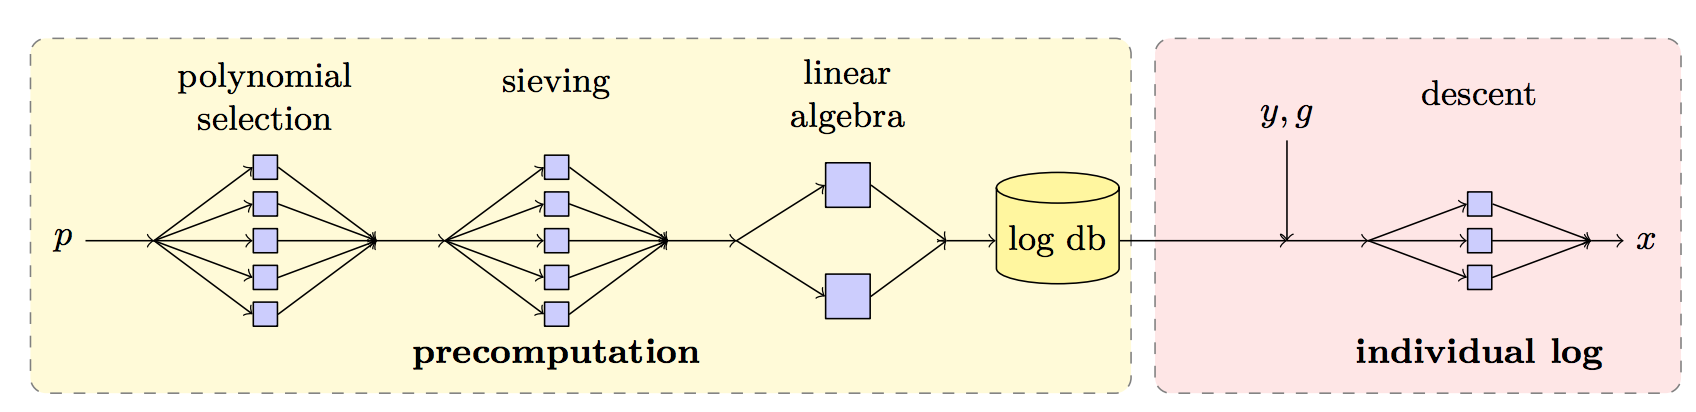
\includegraphics[width=0.8\columnwidth]{graphics/DLOGalg.png}
\end{figure}

\begin{itemize}
\item Algorithm known in mathematical crypto communities since 1990s.
\item Only step 4 uses $y,g$.
\item Precompute database of logarithms of small primes, factor $y$ into
      primes, then compute composite logarithms.
\item Precomputation feasible for 512-bit $p$.
\end{itemize}

\end{frame}

%%%%%%%%%%%%%%%%%%%%%%%%%%%%%%%%%%%%%%%%%%%%%%%%%%%%%%%%%%%%%%%%%%%%%%%%%%%%%%%

\begin{frame}{TLS}

Crypto-suite negotiation:
\begin{figure}
\centering
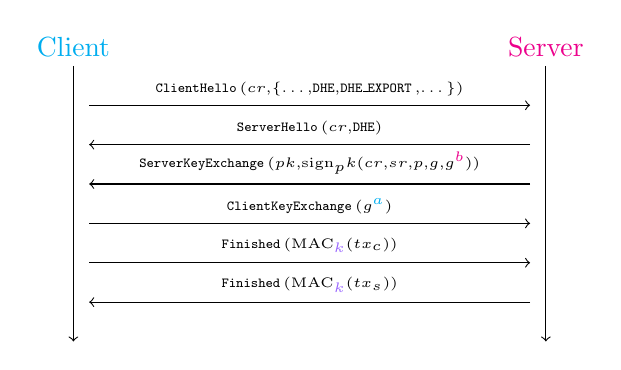
\begin{tikzpicture}

\node[above] (clientStart) at (0,3.5) {\cyan{Client}};
\node[above] (serverStart) at (6,3.5) {\magenta{Server}};
\draw[->]         (0,3.5) -- (0,0);
\draw[->]         (6,3.5) -- (6,0);

\draw[->] (0.2,3) -- (5.8,3)
        node[pos=0.5,above]{\tiny\clienthello($cr$,\{\dots,\dhe,\dheexport,\dots\})};
\draw[->] (5.8,2.5) -- (0.2,2.5)
        node[pos=0.5,above]{\tiny\serverhello($cr$,\dhe)};
\draw[->] (5.8,2) -- (0.2,2)
        node[pos=0.5,above]{\tiny\serverkex($pk$,$\text{sign}_pk$($cr$,$sr$,$p$,$g$,$g^{\magenta{b}}$))};
\draw[->] (0.2,1.5) -- (5.8,1.5)
        node[pos=0.5,above]{\tiny\clientkex($g^{\cyan{a}}$)};
\draw[->] (0.2,1) -- (5.8,1)
        node[pos=0.5,above]{\tiny\finished($\text{MAC}_{\purple{k}}$($tx_c$))};
\draw[->] (5.8,0.5) -- (0.2,0.5)
        node[pos=0.5,above]{\tiny\finished($\text{MAC}_{\purple{k}}$($tx_s$))};

\end{tikzpicture}
\end{figure}

\begin{itemize}
\item \dhe,\dheexport: 1024-/512-bit DH
\item $cr$,$sr$:       Client/server nonces
\item $pk$:            Server's TLS long-term public key
\item $tx_c,tx_s$:     Client's/server's transcript of interaction up to
                       \finished messages
\end{itemize}

\end{frame}

%%%%%%%%%%%%%%%%%%%%%%%%%%%%%%%%%%%%%%%%%%%%%%%%%%%%%%%%%%%%%%%%%%%%%%%%%%%%%%%

\section{Techniques}

%%%%%%%%%%%%%%%%%%%%%%%%%%%%%%%%%%%%%%%%%%%%%%%%%%%%%%%%%%%%%%%%%%%%%%%%%%%%%%%

\begin{frame}{Logjam}

\begin{figure}
\centering
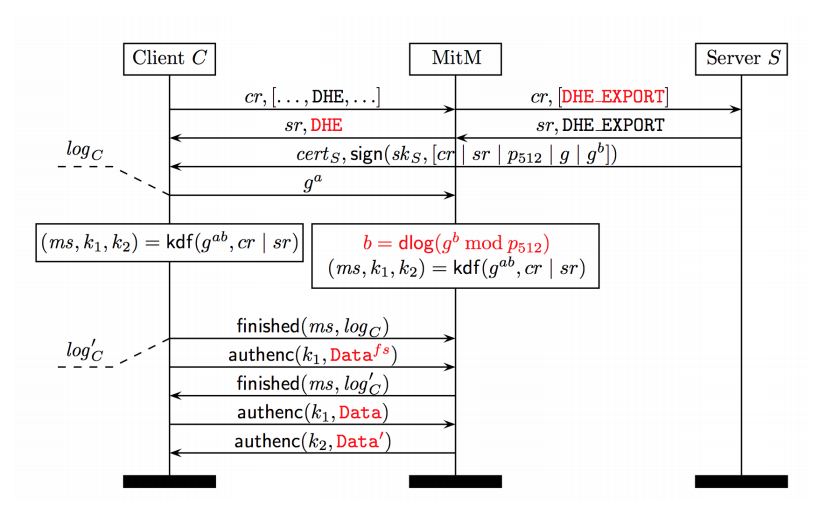
\includegraphics[width=0.6\columnwidth]{graphics/logjam.png}
\end{figure}

\begin{itemize}
\item Eve sits between client and server.
\item Rewrites \clienthello with just \dheexport.
\item Rewrites \serverhello with \dhe: The suite in \serverkex isn't signed.
\item If Eve can compute client exponent $b$, she can forge \finished exchange.
\end{itemize}

\end{frame}

%%%%%%%%%%%%%%%%%%%%%%%%%%%%%%%%%%%%%%%%%%%%%%%%%%%%%%%%%%%%%%%%%%%%%%%%%%%%%%%

\begin{frame}{Attacking Diffie-Hellman}

Authors consider two types of attack
\begin{itemize}
\item Actual attacks on Diffie-Hellman key exchange where
      $|\mathbb{Z}_p^*| \approx 2^{512}$
\item Theoretical attacks against groups of order $2^{768}$ and $2^{1024}$
\end{itemize}
    
\end{frame}

%%%%%%%%%%%%%%%%%%%%%%%%%%%%%%%%%%%%%%%%%%%%%%%%%%%%%%%%%%%%%%%%%%%%%%%%%%%%%%%

\begin{frame}{Man-in-the-Middle}

\begin{figure}
\centering
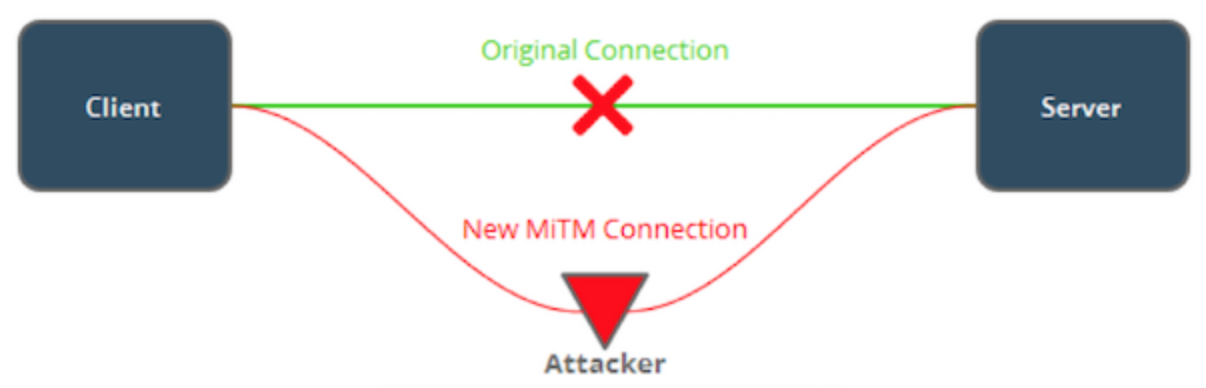
\includegraphics[width=0.86\columnwidth]{graphics/mitm.png}
\end{figure}

\begin{itemize}
\item Web Browser
\item TLS (Transport Layer Security)
\item Server that supports Diffie-Hellman
\end{itemize}
    
\end{frame}

%%%%%%%%%%%%%%%%%%%%%%%%%%%%%%%%%%%%%%%%%%%%%%%%%%%%%%%%%%%%%%%%%%%%%%%%%%%%%%%

\begin{frame}{Man-in-the-Middle}

What do authors target?
\begin{itemize}
\item Servers support old protocols which aren't cryptographically secure
      against modern resources. Therefore, we force the use of unsafe crypto.
\item Length of handshake. If handshake is allowed to take a while (30--200
      seconds) then they can use precomputed data to allow for DLOGs quick
      enough to not trigger a warning or raise suspicion.
\end{itemize}

\end{frame}

%%%%%%%%%%%%%%%%%%%%%%%%%%%%%%%%%%%%%%%%%%%%%%%%%%%%%%%%%%%%%%%%%%%%%%%%%%%%%%%

\begin{frame}{Man-in-the-Middle}

\begin{figure}
\centering
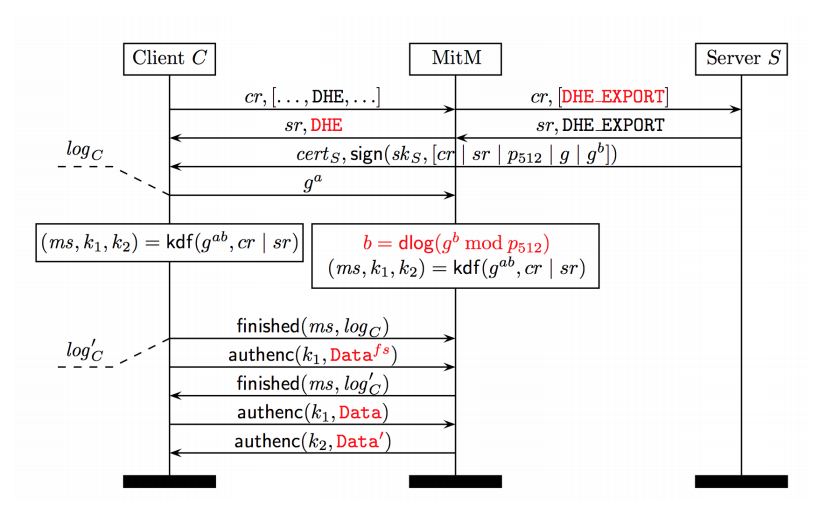
\includegraphics[width=0.8\columnwidth]{graphics/logjam.png}
\end{figure}

\begin{itemize}
\item Signature doesn't include which ciphersuite is used.
\item Adversary attempts to compute shared secrete $g^{ab}$ before handshake
      completes so they can send a \texttt{FINISHED} message in time. Median of
      70 seconds. Can then impersonate server.
\end{itemize} 

\end{frame}

%%%%%%%%%%%%%%%%%%%%%%%%%%%%%%%%%%%%%%%%%%%%%%%%%%%%%%%%%%%%%%%%%%%%%%%%%%%%%%%

\begin{frame}{Man-in-the-Middle}

Browser-Clients
\begin{itemize}
\item Browsers often have short handshake timers
\item Can issue $TLS-Warning Alert$ which resets handshake timer but are
      otherwise ignored by the browser. Firefox in particular can have the
      handshake last indefinitely in this manner. 
\item Will cause connection to hang, but if adversary is hijacking a
      background resource, page will render quickly.
\end{itemize}
Non-Browser Clients (such as from a terminal)
\begin{itemize}
\item Different time limits on handshake, upon which they kill connection.
\item However, commands such as $curl$ or $git$ run unattended and thus have
      long timeouts or none at all. These can be used for hijacking.
\end{itemize}

\end{frame}

%%%%%%%%%%%%%%%%%%%%%%%%%%%%%%%%%%%%%%%%%%%%%%%%%%%%%%%%%%%%%%%%%%%%%%%%%%%%%%%

\begin{frame}{Man-in-the-Middle}

Ephemeral Key Caching
\begin{itemize}
\item Even if DHE is used, often times $g^b$ will be used multiple
      times over the course of multiple handshakes. 
\item Must set flag \texttt{SSL\_OP\_SINGLE\_DH\_USE} for fresh exponents.
      They give many examples of servers which don't, i.e. OpenSSL uses
      $g^b$ over the lifetime of a TLS context.
\item Allows adversary to pre-compute the discrete log.
\item By randomly sampling IPv4 hosts serving browser-trusted certificates
      supporting DHE, 17\% reused $g^b$ at least once over the
      course of 20 handshakes, and 15\% used only one $g^b$.
\end{itemize}

\end{frame}

%%%%%%%%%%%%%%%%%%%%%%%%%%%%%%%%%%%%%%%%%%%%%%%%%%%%%%%%%%%%%%%%%%%%%%%%%%%%%%%

\begin{frame}{Bad DHE}

Even if DHE is used and handshakes are short, there are still issues\\

TLS False Start
\begin{itemize}
\item Reduces connection latency by allowing client to send application data
      early, such as an HTTP request, before handshake is finished with server.
\item Thus, MITM can record the handshake and decrypt the False Start payload at
      their leisure.
\item Firefox 34, Chrome 41, and Windows 10 Internet Explorer send False Start
      with DHE. Initial data often can include sensitive user authentication
      information, such as passwords and cookies.
\end{itemize}

\end{frame}

%%%%%%%%%%%%%%%%%%%%%%%%%%%%%%%%%%%%%%%%%%%%%%%%%%%%%%%%%%%%%%%%%%%%%%%%%%%%%%%

\begin{frame}{Bad DHE}
    
Found evidence of 512-bit primes in non export-DHE. 

Could be a passive eavesdropper instead of MITM, as don't need to force the
server to use export-DHE. 
\begin{itemize}
\item Found 2,631 servers with browser-trusted certificates that used 512-bit
      or weaker primes for non-export-DHE.
\item Decrypted test connections to www.fbi.gov which used default 512-bit DH
      group from OpenSSL.
\end{itemize}

\end{frame}

%%%%%%%%%%%%%%%%%%%%%%%%%%%%%%%%%%%%%%%%%%%%%%%%%%%%%%%%%%%%%%%%%%%%%%%%%%%%%%%

\begin{frame}{Bad DHE}

Vulnerable if subgroups are composite.
\begin{itemize}
\item $|\mathbb{Z}_p^*| = p-1 = 2 \cdot \frac{p-1}{2}$, unless $p =3$. A prime
      $p$ is safe if $\frac{p-1}{2}$ is prime. If not, it's called composite.
\item $g^x$ safe for $x \in [160, 224]$ bits. Unsafe if $g$ has small factors.
\item Carried out attack in the wild using factoring method called Bernstein's
      Batch Factoring. After 5 days of computation across parallelized 28 cores,
      found 36,447 prime factors.
\item Ran Pohlig-Hellman and Pollard lambda on this info which allowed them to
      take the DLOG with time delay hardly noticeable for browser users.
\item Learned exponent info from 460 servers, and learned exactly exponent in
      159 hosts, 53 of which authenticated with valid browser-trusted
      certificates.
\end{itemize}

\end{frame}

%%%%%%%%%%%%%%%%%%%%%%%%%%%%%%%%%%%%%%%%%%%%%%%%%%%%%%%%%%%%%%%%%%%%%%%%%%%%%%%

\begin{frame}{Bad DHE}

Sometimes groups are instantiated incorrectly
\begin{itemize}
\item Digital Signature Algorithm (DSA) has primes $p$ such that $p-1$ has a
      large prime factor $q$, and $g$ only generates subgroup of order $q$.
      These are safe for DH key exchange.
\item Some uses of third-party DSA packages for Java's included hosts who
      accidentally used $q$ as their generator. Subgroup generated by $q$ will
      likely be composite. For this package in particular, leaks 290-bits of
      information about exponents. Can't fully recover exponent, but
      significantly lowers security.
\end{itemize}

\end{frame}

%%%%%%%%%%%%%%%%%%%%%%%%%%%%%%%%%%%%%%%%%%%%%%%%%%%%%%%%%%%%%%%%%%%%%%%%%%%%%%%

\begin{frame}{Theoretical Attacks}

These were all attacks on unsafe crypto, or groups with unsuitable parameter
choices. What if we can't downgrade protocols, and we're using them with strong
groups?
\begin{itemize}
\item 768-bit groups are vulnerable against academic computational resources.
\item There exist a small number of 1024-bit groups which they argue are
      vulnerable against special purpose machines which are within nation-state
      resources. Doesn't require any further academic or algorithmic
      improvements.
\end{itemize}

\end{frame}

%%%%%%%%%%%%%%%%%%%%%%%%%%%%%%%%%%%%%%%%%%%%%%%%%%%%%%%%%%%%%%%%%%%%%%%%%%%%%%%

\begin{frame}{Theoretical Attacks}

Author's examine attacks against standard internet protocols
\begin{itemize}
\item IKE (Internet Key Exchange), SSH (Secure Shell), and TLS (Transport Layer
      Security)
\item Although more expensive than breaking RSA encryption, this payoff is much
      more important, as breaking one 1024-bit prime could compromise millions
      of hosts who use the same parameters for their Diffie-Hellman groups.
\item Possible that NSA is already doing this due to leaked info from Edward
      Snowden showing what NSA has capability of breaking VPN. Better
      explanation than alternatives such as their ability to break RC4 (Rivest
      Cipher 4), AES (Advanced Encryption Standard). 
\end{itemize}

\end{frame}

%%%%%%%%%%%%%%%%%%%%%%%%%%%%%%%%%%%%%%%%%%%%%%%%%%%%%%%%%%%%%%%%%%%%%%%%%%%%%%%

\begin{frame}{Theoretical Attacks}

\begin{figure}
\centering
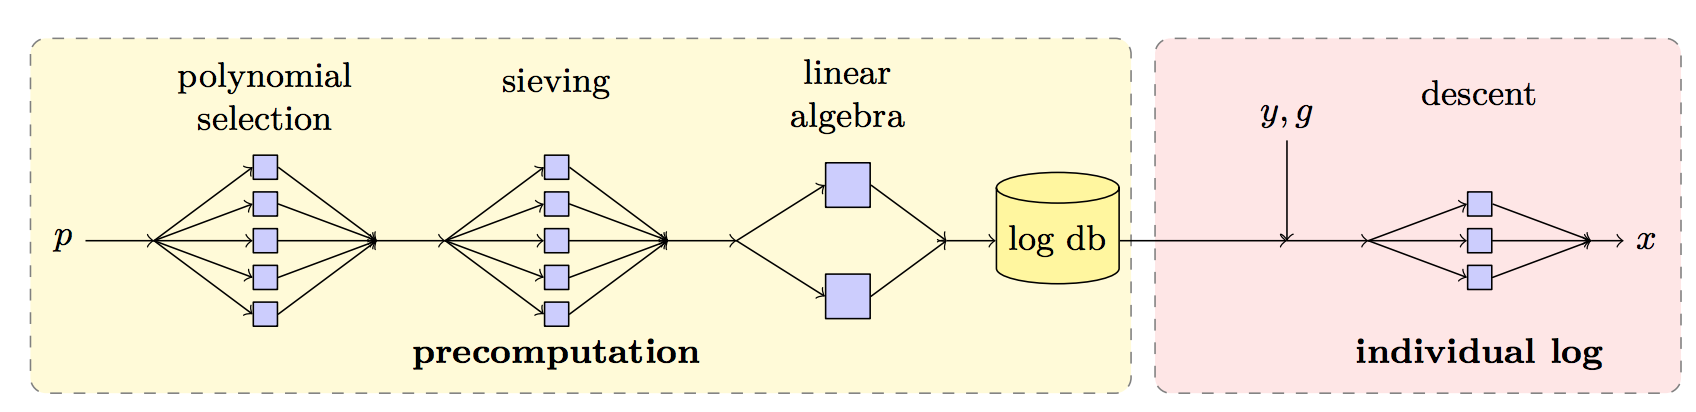
\includegraphics[width=0.86\columnwidth]{graphics/DLOGalg.png}
\end{figure}

\begin{figure}
\centering
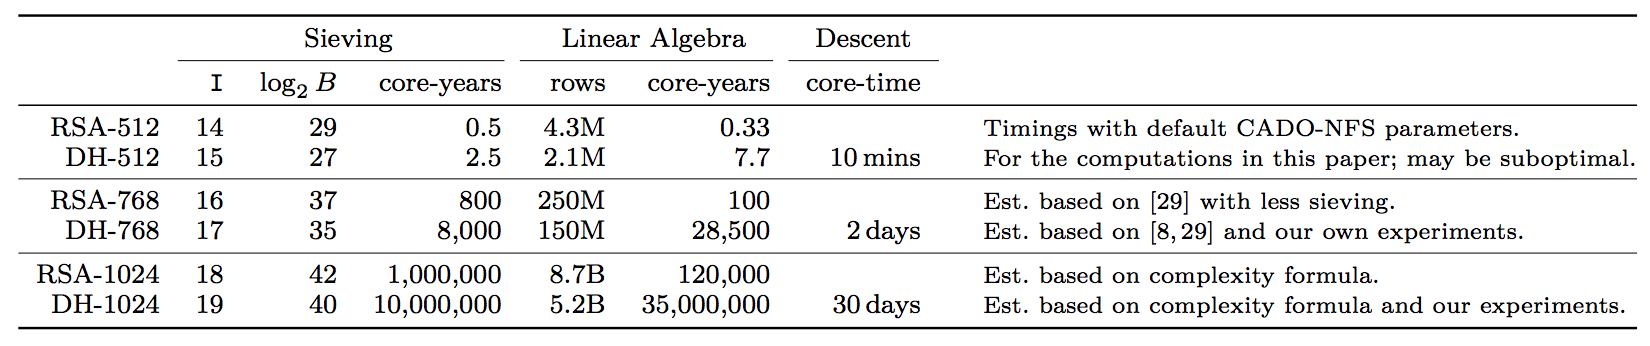
\includegraphics[width=0.86\columnwidth]{graphics/DLOGtable.png}
\end{figure}

Sieving is much more parallelizable than linear algebra step. The more sieving
that's done, the faster the linear algebra step is.

1024-bit info based mainly on asymptotic complexity of sieving algorithm, rather
than actual experimental results.

\end{frame}

%%%%%%%%%%%%%%%%%%%%%%%%%%%%%%%%%%%%%%%%%%%%%%%%%%%%%%%%%%%%%%%%%%%%%%%%%%%%%%%

\begin{frame}{Theoretical Attacks}

Cost of 1024-bit DHE precomputation is 45M core years of work.
\begin{itemize}
\item Sieving: 3M chips could complete sieving in one year. At \$2 a chip,
      and roughly $\$$2M in other required expenses, this would be an \$8M
      investment into ASICs processors.
\item Linear Algebra: Titan supercomputer has 300,000 CPU cores. This would
      take 117 years to complete linear algebra precomputation. At \$94M per
      Titan, this would take \$11B in supercomputers to complete Linear
      Algebra precomputation in 1 year. May be possible to change CPU usage
      to ASICs usage, which would cut down cost by a factor of 80. Thus,
      only cost 100s of millions. 
\item In 2013 the U.S. Consolidated Cryptologic, which includes NSA, had a
      budget of \$10.5B. They prioritize investing in ``groundbreaking
      cryptanalytic capabilities to defeat adversarial cryptography and exploit
      internet traffic.'' Departments ``cryptanalytic IT services'' Received
      budget of \$247M, and ``cryptanalysis and exploitation services program
      C'' received \$360M. 
\end{itemize}

\end{frame}

%%%%%%%%%%%%%%%%%%%%%%%%%%%%%%%%%%%%%%%%%%%%%%%%%%%%%%%%%%%%%%%%%%%%%%%%%%%%%%%

\begin{frame}{NSA}

We know NSA has broken VPN traffic. They argue it's likely that NSA has broken
the DH key exchange portion of the protocol. 

Given oracle which can solve DLOG, all that's needed is one of the following
\begin{itemize}
\item A complete two-sided IKE transcript, $g^a$, $g^b$ , nonces and cookies
      transmitted from both sides
\item For IKEv1, the pre-shared keys used in deriving SKEYID
\end{itemize}

Based off of leaked documents, we know that NSA has this information in VPN
attack network.

\end{frame}

%%%%%%%%%%%%%%%%%%%%%%%%%%%%%%%%%%%%%%%%%%%%%%%%%%%%%%%%%%%%%%%%%%%%%%%%%%%%%%%

\begin{frame}{Effect of a 1024-bit break}

\begin{figure}
\centering
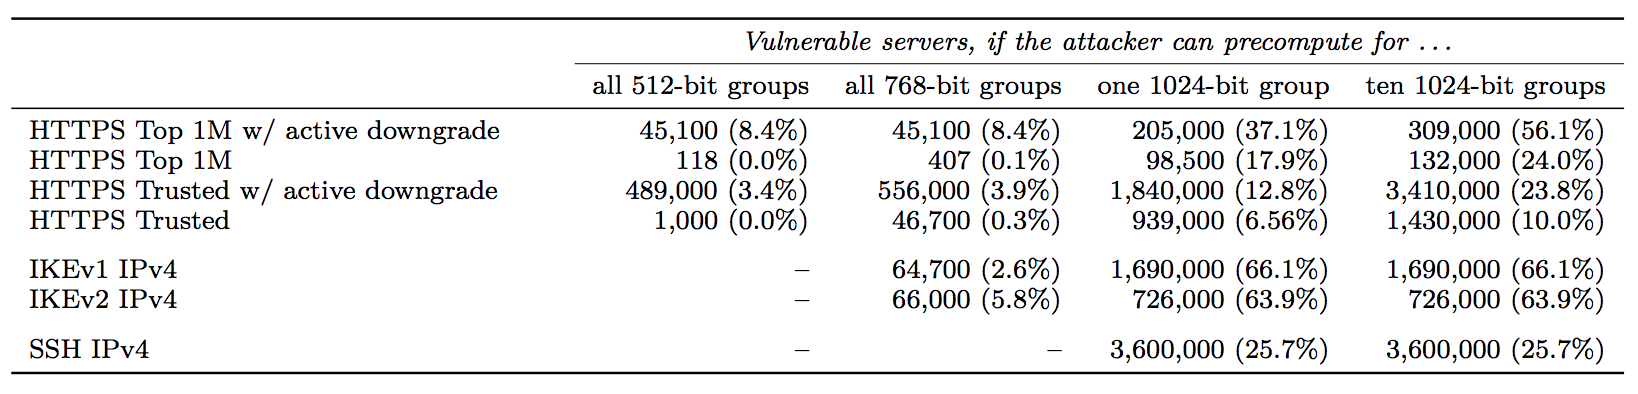
\includegraphics[width=\columnwidth]{graphics/Vulnerabilites.png}
\end{figure}

\begin{itemize}
\item From May 2015, a random sample of 1\% of the IPv4 address space for
      IKEv1 and IKEv2
\item From April 2015, a random sample of 1\% of the IPv4 address space for
      SSH key exchange using DH
\item HTTPS commonly uses DHE
\item TLS is used for to secure email transport
\end{itemize}

\end{frame}

%%%%%%%%%%%%%%%%%%%%%%%%%%%%%%%%%%%%%%%%%%%%%%%%%%%%%%%%%%%%%%%%%%%%%%%%%%%%%%%

\begin{frame}{Solutions}

\begin{figure}
\centering
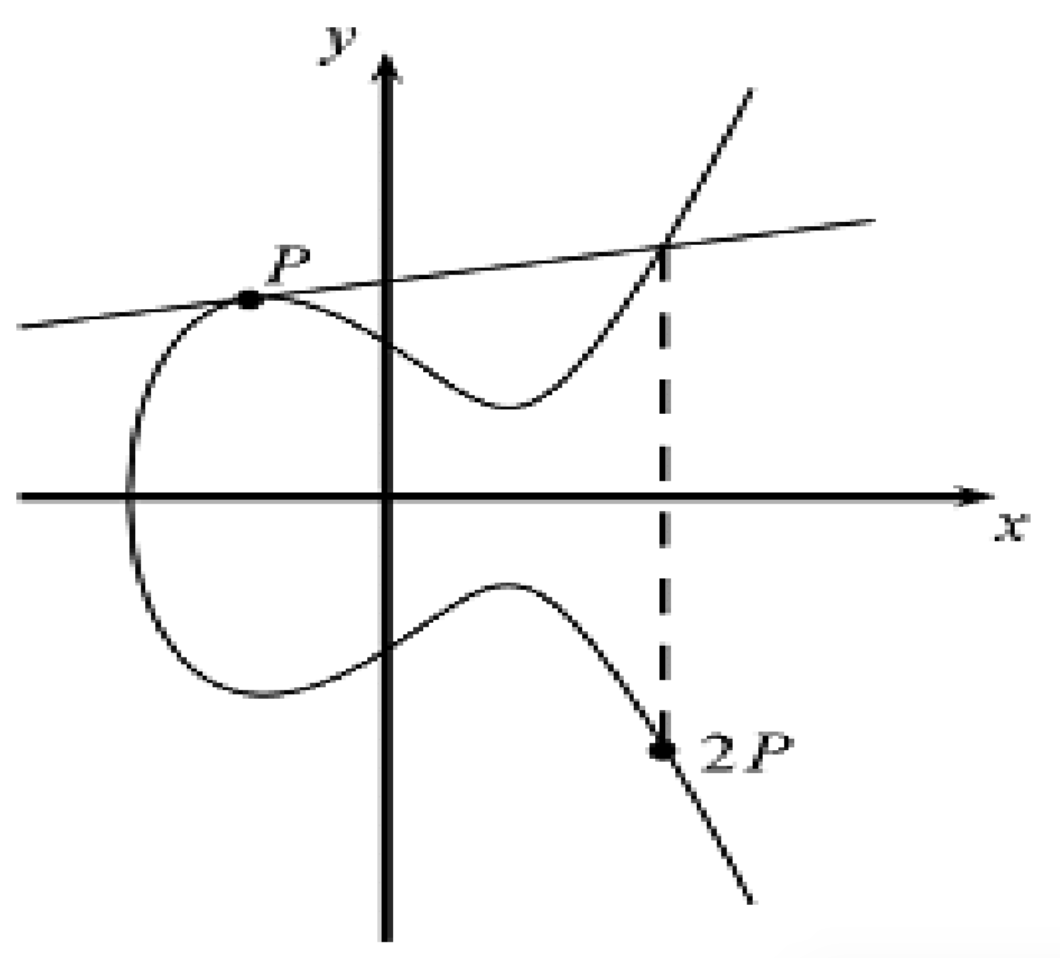
\includegraphics[width=0.6\columnwidth]{graphics/ElipticDH.png}
\end{figure}
    
\end{frame}

%%%%%%%%%%%%%%%%%%%%%%%%%%%%%%%%%%%%%%%%%%%%%%%%%%%%%%%%%%%%%%%%%%%%%%%%%%%%%%%

\begin{frame}{Solutions}

\begin{itemize}
\item Use bigger groups, like 2048 bit primes or larger. NIST recommended 2048
      and higher since 2010. $10^9$ times more difficult, not feasible until
      algorithmic improvement.
\item Ciphersuits should include primes of 1024 bits. 512-bit primes aren't
      secure anymore.
\item Refresh to new groups from time to time if forced to use 1024-bit primes.
\item Security community, please don't deliberately use weak crypto. Export
      crypto existed because it was believed to only be vulnerable to NSA. Now
      vulnerable to academic resources. Always exercise best practices.
\end{itemize}

\end{frame}

%%%%%%%%%%%%%%%%%%%%%%%%%%%%%%%%%%%%%%%%%%%%%%%%%%%%%%%%%%%%%%%%%%%%%%%%%%%%%%%

\begin{frame}{Solutions}

Before Work
\begin{itemize}
\item IE, Chrome, Firefox, Opera accepted 512-bit ptimes
\item Safari allowed groups as small as 16 bit primes
\item Notified Apachi, Oracle, IBM, Cisco, Akamai, and various other providers
\end{itemize}
After Work
\begin{itemize}
\item IE, Firefox, and Chrome transitioning to minimum of 1024 bit groups.
      OpenSSL and Safari expected to follow suit.
\item Akamai removed export ciphersuites. Many TLS developers plan to support
      well known 2048-bit groups and higher, and to reject weak ones.
\end{itemize}
\end{frame}

%%%%%%%%%%%%%%%%%%%%%%%%%%%%%%%%%%%%%%%%%%%%%%%%%%%%%%%%%%%%%%%%%%%%%%%%%%%%%%%

\begin{frame}{Strengths}

Their result is important. Symmetric-key crypto is vital to modern security.
Shows that the fundamental building block of key exchange is vulnerable.

\end{frame}

%%%%%%%%%%%%%%%%%%%%%%%%%%%%%%%%%%%%%%%%%%%%%%%%%%%%%%%%%%%%%%%%%%%%%%%%%%%%%%%

\begin{frame}{Weakness}

Didn't discuss how much of anything worked. Everything was so high-level that I
didn't feel like I really learned anything beyond the results of their study.

\end{frame}

%%%%%%%%%%%%%%%%%%%%%%%%%%%%%%%%%%%%%%%%%%%%%%%%%%%%%%%%%%%%%%%%%%%%%%%%%%%%%%%

\begin{frame}{Synthesis}

\only<1>{
Is it possible to construct a honeypot for FBI which could prove that
they have the ability to break 1024-bit DHE?
}
\only<2>{
Quantum precomputation: Could a quantum algorithm be used to efficiently
generate the prime-logarithm DB, leaving the descent step for a classical
computer?
}

\end{frame}

%%%%%%%%%%%%%%%%%%%%%%%%%%%%%%%%%%%%%%%%%%%%%%%%%%%%%%%%%%%%%%%%%%%%%%%%%%%%%%%

\begin{frame}{Questions?}
\end{frame}

%%%%%%%%%%%%%%%%%%%%%%%%%%%%%%%%%%%%%%%%%%%%%%%%%%%%%%%%%%%%%%%%%%%%%%%%%%%%%%%

\end{document}
